%%%%% Design %%%%%
\section{Design} 
This is the Design of the final report.
\subsection{Methodology}
\subsubsection{Forward Kinematics}
The manipulator consists of four units, and the backbones of each section are perpendicular to each other. To derive the 
workspace of the manipulator for further analysis, the forward kinematics formula need to be conducted. According to the 
fishbone continuum robot\cite{fishboneCR}, the forward kinematics formula of two perpendicular units are shown in 
Equations \ref{eq:x_coordinate}, \ref{eq:y_coordinate}, and \ref{eq:z_coordinate}.
\begin{align}
    &\begin{aligned}
    x=&-\frac{S_{r}r}{\Delta S_{1}}+\frac{S_{r}r}{\Delta S_{1}}\cos\left(\frac{\Delta S_{l}}{r}\right)-d_{1}\sin\left(\frac{\Delta S_{l}}{r}\right) \\
    &-\frac{S_{r}r}{\Delta S_{3}}\sin\left(\frac{\Delta S_{1}}{r}\right)\sin\left(\frac{\Delta S_{3}}{r}\right)-d_{2}\sin\left(\frac{\Delta S_{1}}{r}\right)\cos\left(\frac{\Delta S_{3}}{r}\right) 
    \end{aligned}
    \label{eq:x_coordinate} \\
    &\begin{aligned}
        y=-\frac{S_rr}{\Delta S_3}+\frac{S_rr}{\Delta S_3}\cos\left(\frac{\Delta S_3}{r}\right)-d_2\sin\left(\frac{\Delta S_3}{r}\right)
    \end{aligned}
    \label{eq:y_coordinate} \\
    &\begin{aligned}
        \text{z} =&\frac{S_{r}r}{\Delta S_{1}}\sin\left(\frac{\Delta S_{\mathrm{l}}}{r}\right)+d_{1}\cos\left(\frac{\Delta S_{\mathrm{l}}}{r}\right) \\
        +&\frac{S_{r}r}{\Delta S_{3}}\sin\left(\frac{\Delta S_{3}}{r}\right)\cos\left(\frac{\Delta S_{1}}{r}\right)+d_{2}\cos\left(\frac{\Delta S_{1}}{r}\right)\cos\left(\frac{\Delta S_{3}}{r}\right). 
    \end{aligned}
    \label{eq:z_coordinate}
\end{align}
However, calculating the centroid directly using the above formula becomes complex while there are four units in the manipulator. 
Additionally, the inverse kinematics part also requires the derivation of corresponding matrices for subsequent calculations 
using the composite coordinate transformation formula. Therefore, The relevant matrices for subsequent calculations need to 
be derived. \\
According to the design specifications, the manipulator comprises four units. The backbones of the units are vertically aligned. 
The base coordinate system can be established with the centroid of base disk upper surface serving as the origin. The x-axis of 
the coordinate system is aligned with the backbone of the unit nearest to the base disk. Consequently, the backbones of units 1 
and 3 are parallel to the x-axis, while those of units 2 and 4 are parallel to the y-axis. The positions of the five centroids 
in the base coordinate system when the manipulator is in the initial position are shown in Figure \ref{fig:kinematics model 0_0_0_0}. 
The centroids of the five disc upper surfaces are designated as $node_1$, $node_2$, $node_3$, $node_4$, and $node_5$. \\
\begin{figure}[H] %[H] "corresponds to start the figure Here" 
    \centering %alignment can be flushleft or flushright
    \captionsetup{labelsep=colon}
    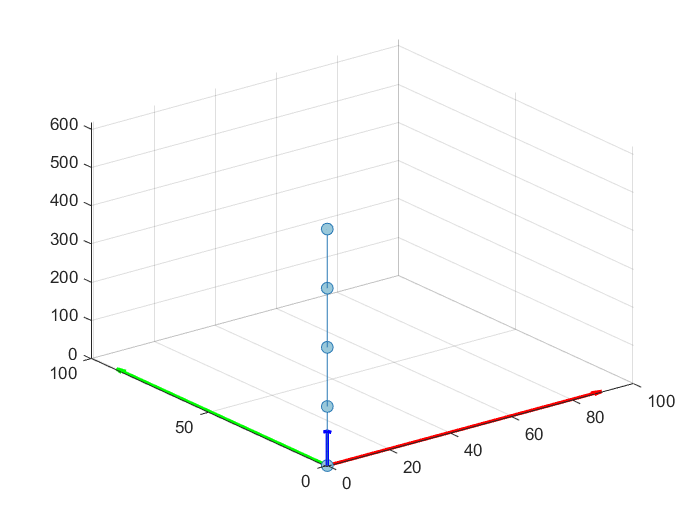
\includegraphics[width=1.0\textwidth]{Image/MATLAB/manipulator_0_0_0_0.png} 
    \caption[The kinematics model of manipulator in the initial position]
    {\centering \textit{\textbf{The kinematics model of manipulator in initial position.}}}
    \label{fig:kinematics model 0_0_0_0}
\end{figure}
\noindent The unit 1 is restricted to bending in the y-z plane of the coordinate system where $node_1$ serves as the origin, 
while the unit 2 is restricted to bending in the x-z plane of the coordinate system where $node_2$ serves as the origin. 
Similarly, the unit 3 and unit 4 are subject to the same constraints. The bending angles for these units are defined as 
$\alpha_1$, $\alpha_2$, $\alpha_3$, and $\alpha_4$, respectively. The positions of the manipulator model in the base coordinate 
system after bending each unit by $90 \degree$ are illustrated in Figure \ref{fig:kinematics_model_resp}.
\begin{figure}[H] %[H] "corresponds to start the figure Here" 
    \centering %alignment can be flushleft or flushright
    \captionsetup{labelsep=colon}
    \begin{subfigure}{0.48\textwidth} % subfigure 1
        \centering
        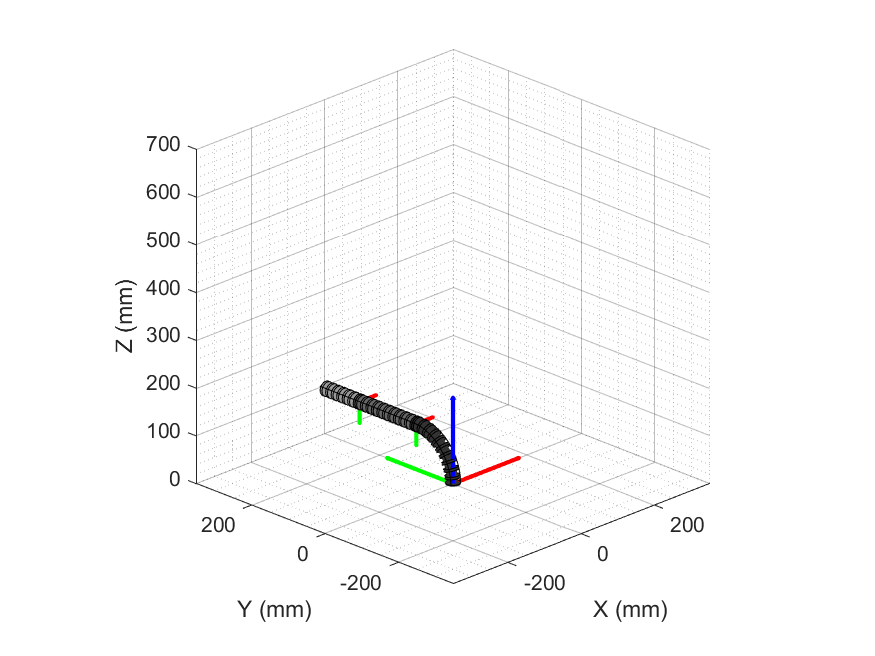
\includegraphics[width=\linewidth]{Image/MATLAB/manipulator_90_0_0_0.png}
        \caption{$\alpha_1=90 \degree,\alpha_2=0,\alpha_3=0,\alpha_4=0$}
    \end{subfigure}
    \hfill
    \begin{subfigure}{0.48\textwidth} % subfigure 2
        \centering
        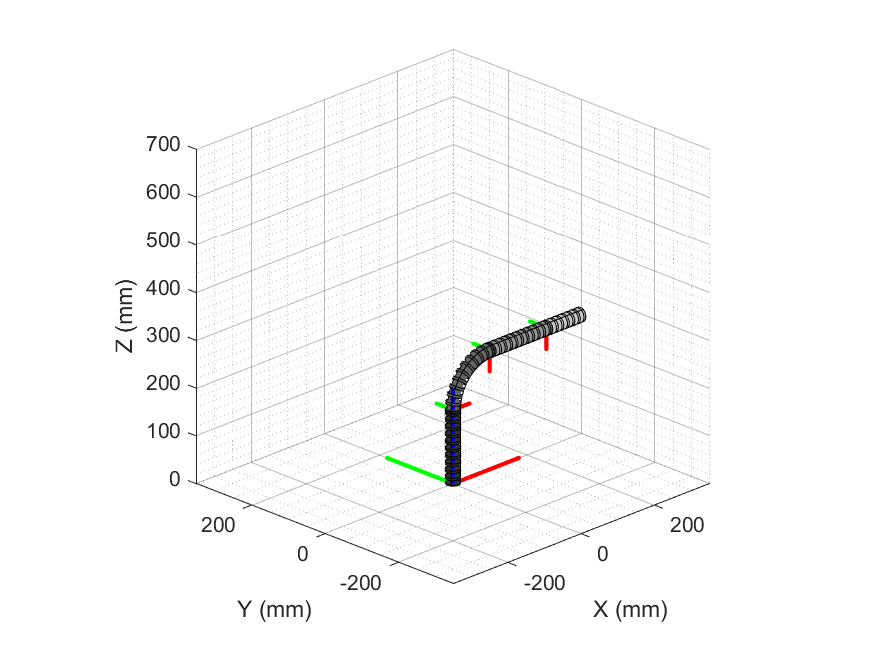
\includegraphics[width=\linewidth]{Image/MATLAB/manipulator_0_90_0_0.png}
        \caption{$\alpha_1=0,\alpha_2=90 \degree,\alpha_3=0,\alpha_4=0$}
    \end{subfigure}
    \begin{subfigure}{0.48\textwidth} % subfigure 3
        \centering
        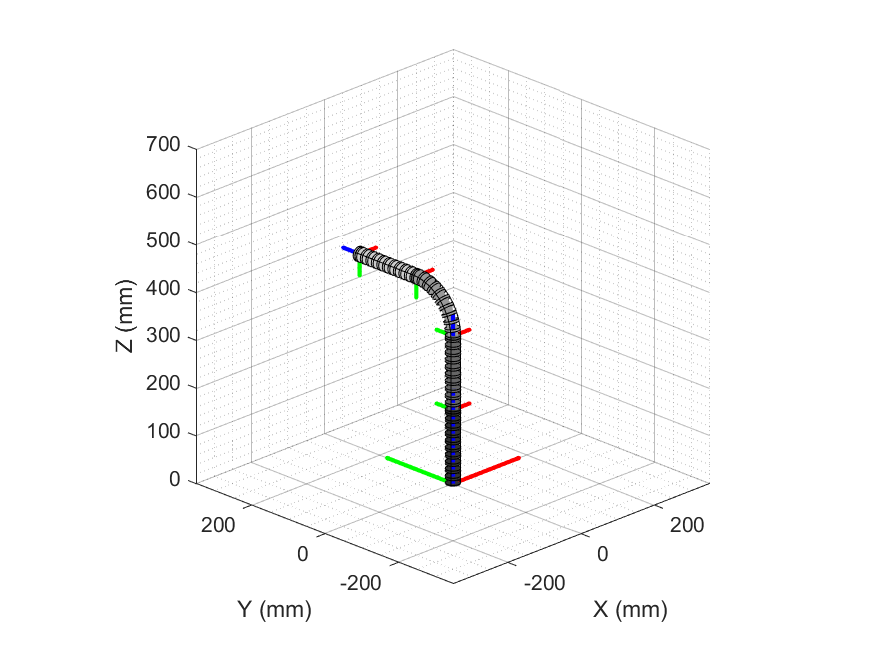
\includegraphics[width=\linewidth]{Image/MATLAB/manipulator_0_0_90_0.png}
        \caption{$\alpha_1=0,\alpha_2=0,\alpha_3=90 \degree,\alpha_4=0$}
    \end{subfigure}
    \hfill
    \begin{subfigure}{0.48\textwidth}
        \centering
        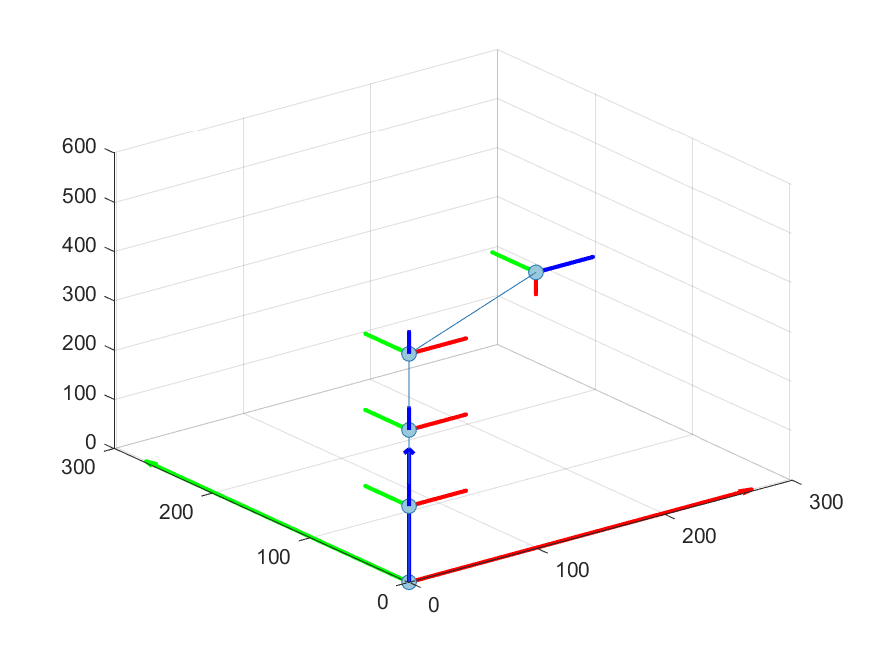
\includegraphics[width=\linewidth]{Image/MATLAB/manipulator_0_0_0_90.png}
        \caption{$\alpha_1=0,\alpha_2=0,\alpha_3=0,\alpha_4=90 \degree$}
    \end{subfigure}
    \caption[The kinematics model of manipulator with respective bending units]
    {\centering \textit{\textbf{The kinematics model of manipulator with respective bending units.}}}
    \label{fig:kinematics_model_resp}
\end{figure}
\noindent While the units bend to the positive direction of x-axis or y-axis, the bending angles $\alpha$ are positive. 
Owing to the distinct properties of the four units, different calculation methods are required for analysis. The unit $i$ 
have a base node $node_i$ and an end effector node $node_{i+1}$. To further calculate the position of $node_{i+1}$ in the 
base coordinate system, these matrices can be employed in the Equation \ref{eq:node i+1 calculation}.
\begin{align}
    &\textbf{P}_{i+1}^{base} = \textbf{R}_{i} \times \textbf{P}_{i+1}^{i} + \textbf{P}_{i}^{base}
    \label{eq:node i+1 calculation}
\end{align}
\begin{align*}
    &\ \textbf{P}_{i+1}^{base}\text{: The position of $node_{i+1}$ in the base coordinate system.}\\
    &\ \textbf{R}_{i}\text{: The rotational matrix tranforms the base coordinate system into coordinate}\\
    &\ \qquad\text{system \textit{i}, which is the coordinate system with origin $node_i$.}\\
    &\ \textbf{P}_{i+1}^{i}\text{: The position of $node_{i+1}$ in coordinate system \textit{i}.}\\
    &\ \textbf{P}_{i}^{base}\text{: The position of $node_{i}$ in the base coordinate system.}
\end{align*}
\begin{itemize}
    \item Unit 1 \\
    For Unit 1, the relationship between the relative position matrix of $node_1$ and $node_2$ $\textbf{P}_{2}^{1}$ and 
    $\alpha_1$ is shown in Equation \ref{eq:node2_postion_relative}.
    \begin{align}
        \textbf{P}_{2}^{1} = 
        \begin{bmatrix}
            0 \\
            (R_1\cdot(1-\cos(\alpha_1)) + d_2\cdot \sin(\alpha_1)) \\
            (R_1\cdot \sin(\alpha_1) + d_2\cdot \cos(\alpha_1)) \\
        \end{bmatrix}&
        \label{eq:node2_postion_relative} \\
        \nonumber (hint: \ R_1 = {Sr}_1/ &\alpha_1)
    \end{align}
    $R_1$ is the radius of the Unit 1 bending curve, ${Sr}_1$ is the length of the Unit 1 backbone, and $d_2$ is the thickness 
    of the disc whose centroid is $node_2$. Meanwhile, the rotational matrix $\textbf{R}_{1}$ and the position matrix of 
    $node_1$ $\textbf{P}_{1}^{base}$ are shown in Equations \ref*{eq:unit1_rotation_matrix} and \ref{eq:node1_position_absolute}.
    \begin{align}
        &\begin{aligned}
            \textbf{R}_{1} = 
            \begin{bmatrix}
                1 & 0 & 0 \\
                0 & 1 & 0 \\
                0 & 0 & 1 \\
            \end{bmatrix}
        \end{aligned}
        \label{eq:unit1_rotation_matrix} \\
        &\begin{aligned}
            \textbf{P}_{1}^{base} = 
            \begin{bmatrix}
                0 & 0 & 0\\
            \end{bmatrix}^{\textbf{T}}
        \end{aligned}
        \label{eq:node1_position_absolute}
    \end{align}
    According to the Equations \ref{eq:node2_postion_relative}, \ref*{eq:unit1_rotation_matrix}, and \ref{eq:node1_position_absolute}, 
    the position matrix of $node_{2}$ in the base coordinate system $\textbf{P}_{2}^{base}$ can be calculated in Equation \ref{eq:node2_position_absolute}.
    \begin{align}
        &\textbf{P}_{2}^{base} = \textbf{R}_{1} \times \textbf{P}_{2}^{1} + \textbf{P}_{1}^{base} \nonumber \\
        &=
        \begin{bmatrix}
            1 & 0 & 0 \\
            0 & 1 & 0 \\
            0 & 0 & 1 \\
        \end{bmatrix}
        \times
        \begin{bmatrix}
            0 \\
            (R_1\cdot(1-\cos(\alpha_1)) + d_2\cdot \sin(\alpha_1)) \\
            (R_1\cdot \sin(\alpha_1) + d_2\cdot \cos(\alpha_1)) \\
        \end{bmatrix}
        +
        \begin{bmatrix}
            0 \\
            0 \\
            0 \\
        \end{bmatrix} \nonumber \\
        &=
        \begin{bmatrix}
            0 \\
            (R_1\cdot(1-\cos(\alpha_1)) + d_2\cdot \sin(\alpha_1)) \\
            (R_1\cdot \sin(\alpha_1) + d_2\cdot \cos(\alpha_1)) \\
        \end{bmatrix}
        \label{eq:node2_position_absolute}
    \end{align}
    \item Unit 2 \\
    For Unit 2, the relationship between the relative position matrix of $node_2$ and $node_3$ $\textbf{P}_{3}^{2}$ and 
    $\alpha_2$ is shown in Equation \ref{eq:node3_postion_relative}.
    \begin{align}
        \textbf{P}_{3}^{2} = 
        \begin{bmatrix}
            (R_2\cdot(1-\cos(\alpha_2)) + d_3\cdot \sin(\alpha_2)) \\
            0 \\
            (R_2\cdot \sin(\alpha_2) + d_3\cdot \cos(\alpha_2)) \\
        \end{bmatrix}&
        \label{eq:node3_postion_relative} \\
        \nonumber (hint: \ R_2 = {Sr}_2/ &\alpha_2)
    \end{align}
    $R_2$ is the radius of the Unit 2 bending curve, ${Sr}_2$ is the length of the Unit 2 backbone, and $d_3$ is the thickness 
    of the disc whose centroid is $node_3$. Meanwhile, the rotational matrix $\textbf{R}_{2}$ and the position matrix of 
    $node_2$ $\textbf{P}_{2}^{base}$ are shown in Equations \ref*{eq:unit2_rotation_matrix} and \ref{eq:node2_position_absolute}.
    \begin{align}
        &\begin{aligned}
            \textbf{R}_{2} = 
            \begin{bmatrix}
                1 & 0 & 0 \\
                0 & \cos(\alpha_1) & \sin(\alpha_1) \\
                0 & -\sin(\alpha_1) & \cos(\alpha_1) \\
            \end{bmatrix}
        \end{aligned}
        \label{eq:unit2_rotation_matrix}
    \end{align}
    According to the Equations \ref{eq:node2_position_absolute}, \ref{eq:node3_postion_relative}, and \ref*{eq:unit2_rotation_matrix}, 
    the position matrix of $node_{3}$ in the base coordinate system $\textbf{P}_{3}^{base}$ can be calculated in Equation \ref{eq:node3_position_absolute}.
    \begin{align}
        &\textbf{P}_{3}^{base} = \textbf{R}_{1} \times \textbf{R}_{2} \times \textbf{P}_{3}^{2} + \textbf{P}_{2}^{base} \nonumber \\
        &= 
        \begin{bmatrix}
            1 & 0 & 0 \\
            0 & 1 & 0 \\
            0 & 0 & 1 \\
        \end{bmatrix}
        \times
        \begin{bmatrix}
            1 & 0 & 0 \\
            0 & \cos(\alpha_1) & \sin(\alpha_1) \\
            0 & -\sin(\alpha_1) & \cos(\alpha_1) \\
        \end{bmatrix} \nonumber \\
        &\times
        \begin{bmatrix}
            (R_2\cdot(1-\cos(\alpha_2)) + d_3\cdot \sin(\alpha_2)) \\
            0 \\
            (R_2\cdot \sin(\alpha_2) + d_3\cdot \cos(\alpha_2)) \\
        \end{bmatrix} \nonumber \\
        &+
        \begin{bmatrix}
            0 \\
            (R_1\cdot(1-\cos(\alpha_1)) + d_2\cdot \sin(\alpha_1)) \\
            (R_1\cdot \sin(\alpha_1) + d_2\cdot \cos(\alpha_1)) \\
        \end{bmatrix}
        \label{eq:node3_position_absolute}
    \end{align}
    \item Unit 3 \\
    For Unit 3, the relationship between the relative position matrix of $node_3$ and $node_4$ $\textbf{P}_{4}^{3}$ and 
    $\alpha_3$ is shown in Equation \ref{eq:node4_postion_relative}.
    \begin{align}
        \textbf{P}_{4}^{3} = 
        \begin{bmatrix}
            0 \\
            (R_3\cdot(1-\cos(\alpha_3)) + d_4\cdot \sin(\alpha_3)) \\
            (R_3\cdot \sin(\alpha_3) + d_4\cdot \cos(\alpha_3)) \\
        \end{bmatrix}&
        \label{eq:node4_postion_relative} \\
        \nonumber (hint: \ R_2 = {Sr}_2/ &\alpha_2)
    \end{align}
    $R_3$ is the radius of the Unit 3 bending curve, ${Sr}_3$ is the length of the Unit 3 backbone, and $d_4$ is the thickness 
    of the disc whose centroid is $node_4$. Meanwhile, the rotational matrix $\textbf{R}_{3}$ and the position matrix of 
    $node_3$ $\textbf{P}_{3}^{base}$ are shown in Equations \ref*{eq:unit3_rotation_matrix} and \ref{eq:node3_position_absolute}.
    \begin{align}
        &\begin{aligned}
            \textbf{R}_{3} = 
            \begin{bmatrix}
                \cos(\alpha_2) & 0 & \sin(\alpha_2) \\
                0 & 1 & 0 \\
                -\sin(\alpha_2) & 0 & \cos(\alpha_2) \\
            \end{bmatrix}
        \end{aligned}
        \label{eq:unit3_rotation_matrix}
    \end{align}
    According to the Equations \ref{eq:node3_position_absolute}, \ref{eq:node4_postion_relative}, and \ref*{eq:unit3_rotation_matrix}, 
    the position matrix of $node_{4}$ in the base coordinate system $\textbf{P}_{4}^{base}$ can be calculated in Equation \ref{eq:node4_position_absolute}.
    \begin{align}
        &\textbf{P}_{4}^{base} = \textbf{R}_{1} \times\textbf{R}_{2} \times\textbf{R}_{3} \times \textbf{P}_{4}^{3} + \textbf{P}_{3}^{base} \nonumber \\
        &= \textbf{R}_{1}\times\textbf{R}_{2}\times
        \begin{bmatrix}
            \cos(\alpha_2) & 0 & \sin(\alpha_2) \\
            0 & 1 & 0 \\
            -\sin(\alpha_2) & 0 & \cos(\alpha_2) \\
        \end{bmatrix} \nonumber \\
        &\times
        \begin{bmatrix}
            0 \\
            (R_3\cdot(1-\cos(\alpha_3)) + d_4\cdot \sin(\alpha_3)) \\
            (R_3\cdot \sin(\alpha_3) + d_4\cdot \cos(\alpha_3)) \\
        \end{bmatrix} + \textbf{P}_{3}^{base}
        \label{eq:node4_position_absolute}
    \end{align}
    \item Unit 4 \\
    In summary, the position matrix of $node_5$ in the base coordinate system $P_5^{base}$can be represented by Equation \ref{eq:node5_position_absolute}.
    \begin{align}
        \textbf{P}_{5}^{base} = \textbf{R}_{1} \times\textbf{R}_{2} \times\textbf{R}_{3} \times\textbf{R}_{4} \times \textbf{P}_{5}^{4} + \textbf{P}_{4}^{base}
        \label{eq:node5_position_absolute}
    \end{align}
\end{itemize}

Applying the corresponding transformations to the Equation \ref{eq:node i+1 calculation} reveals the patterns shown 
in Equations \ref{eq:nodei+1_position_absolute_minus} and \ref{eq:nodei+1_position_absolute}.
\begin{align}
    &\textbf{P}_{i+1}^{base} - \textbf{P}_{i}^{base} = \prod_{n=1}^{i}\textbf{R}_{n}\times \textbf{P}_{i+1}^{i} 
    \label{eq:nodei+1_position_absolute_minus} \\
    &\textbf{P}_{i+1}^{base} = \sum_{m=1}^{i}\left[\prod_{n=1}^{m}\textbf{R}_{n}\times \textbf{P}_{m+1}^{m}\right] \quad(\textbf{P}_{1}^{base} = 0)
    \label{eq:nodei+1_position_absolute}
\end{align}

\begin{figure}[H] %[H] "corresponds to start the figure Here" 
    \centering %alignment can be flushleft or flushright
    \captionsetup{labelsep=colon}
    \begin{subfigure}{0.9\textwidth} % subfigure 1
        \centering
        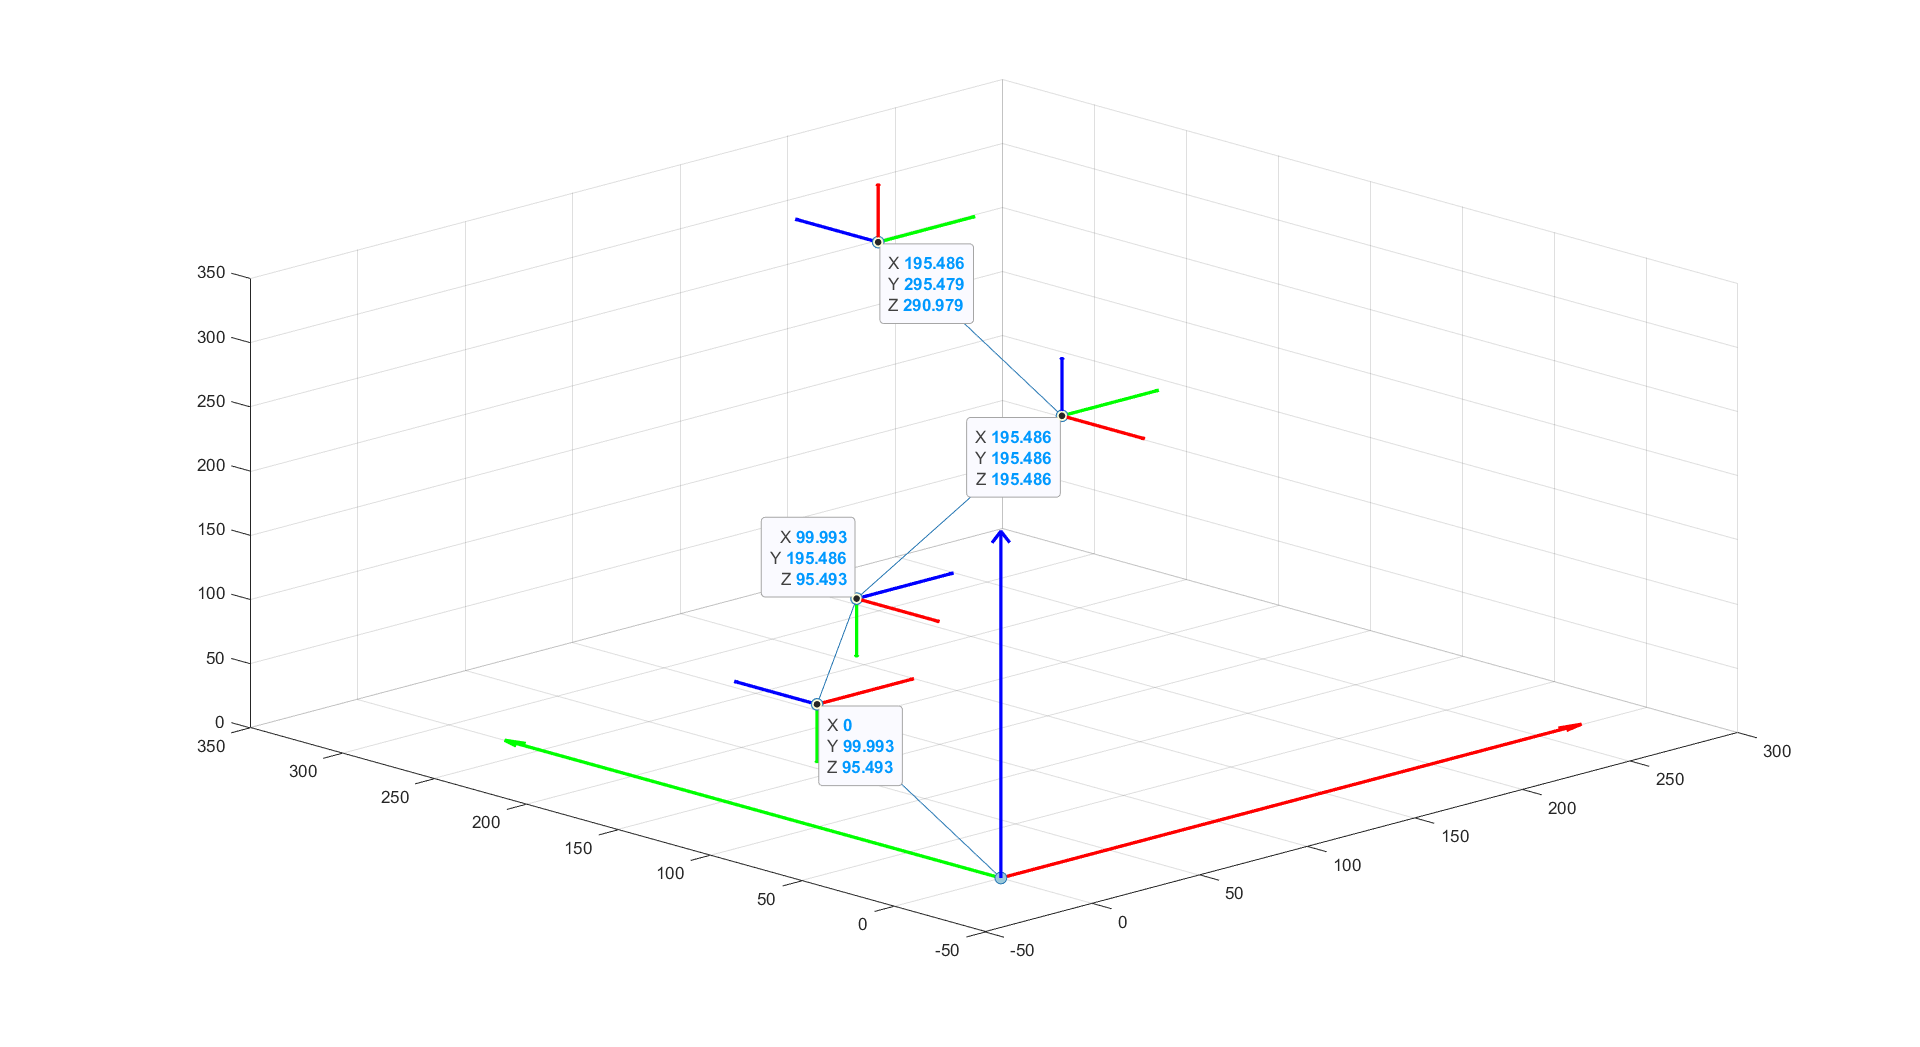
\includegraphics[width=\linewidth]{Image/MATLAB/manipulator_90_90_-90_-90.png}
        \caption{$\alpha_1=90\degree,\alpha_2=90\degree,\alpha_3=-90\degree,\alpha_4=-90\degree$}
    \end{subfigure}
    \hfill
    \begin{subfigure}{0.9\textwidth} % subfigure 2
        \centering
        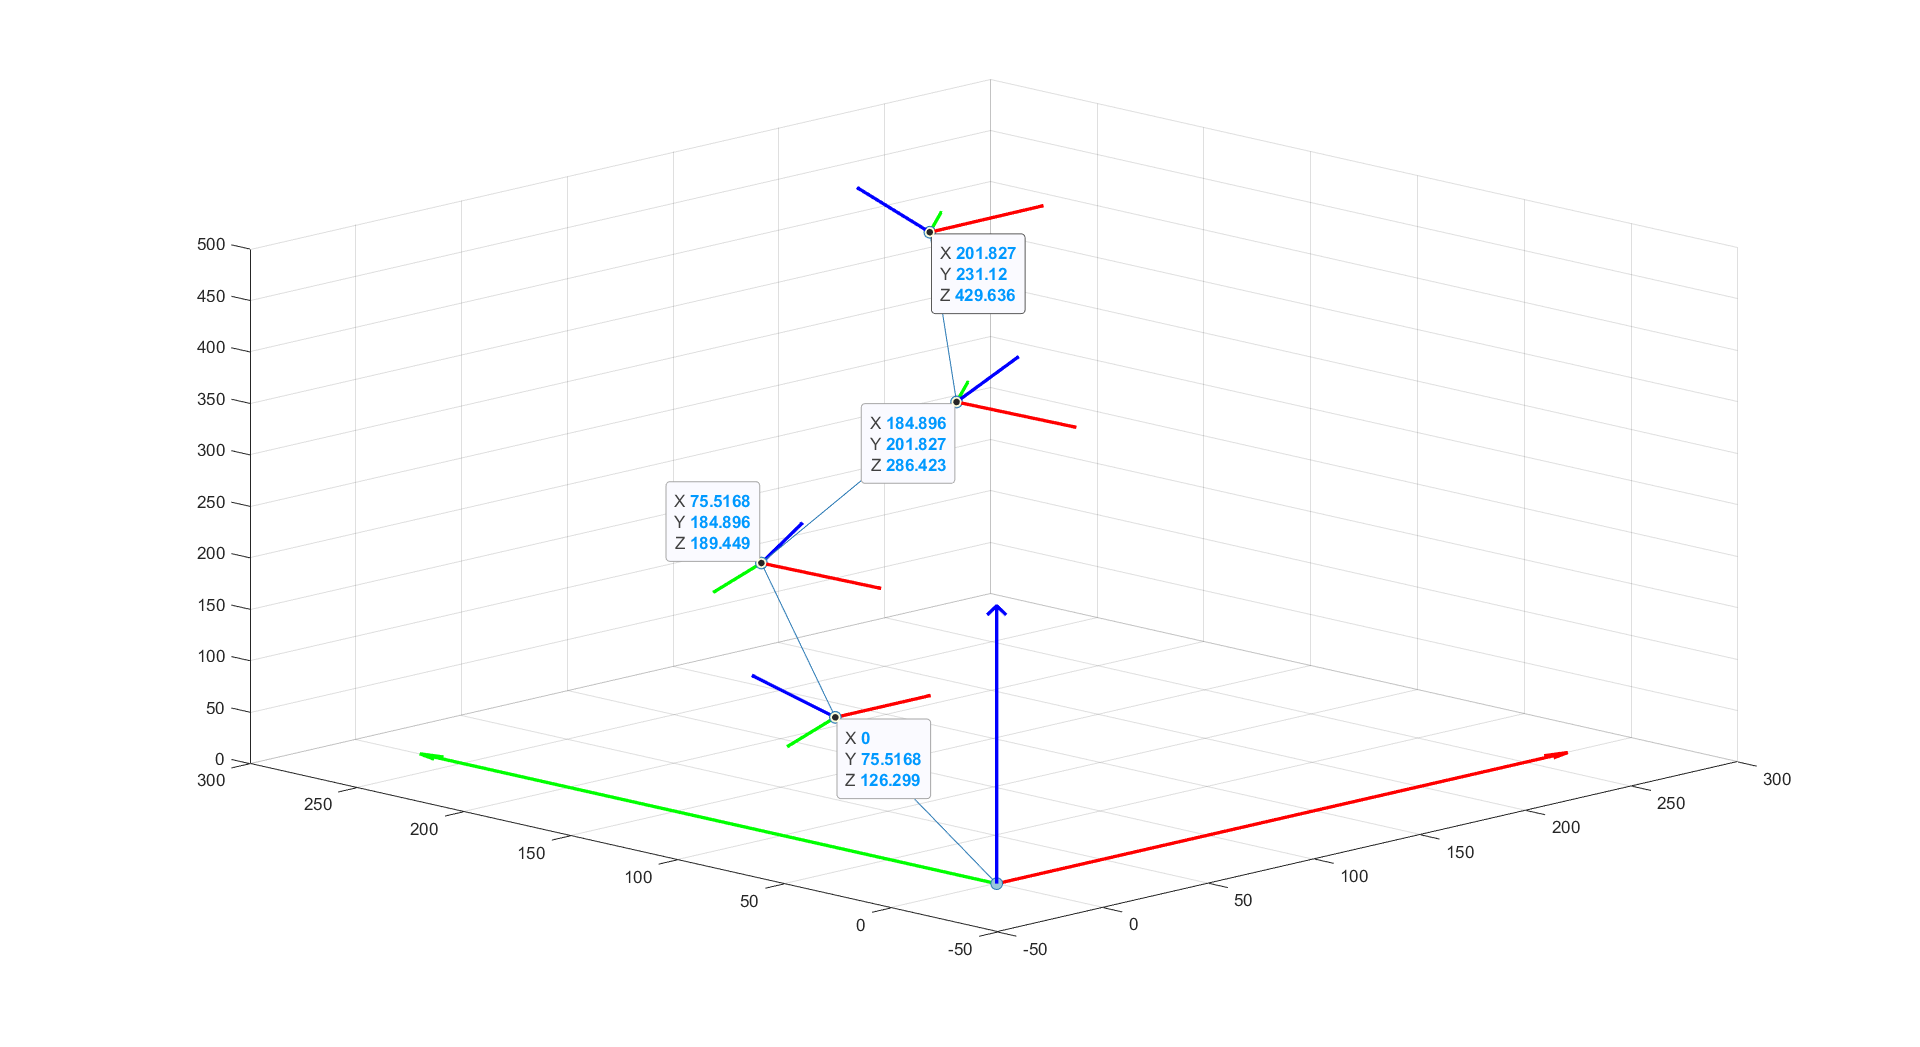
\includegraphics[width=\linewidth]{Image/MATLAB/manipulator_60_60_-60_-60.png}
        \caption{$\alpha_1=60\degree,\alpha_2=60 \degree,\alpha_3=-60\degree,\alpha_4=-60\degree$}
    \end{subfigure}
    \caption[The kinematics model of manipulator with respective bending units]
    {\centering \textit{\textbf{The kinematics model of manipulator with respective bending units.}}}
    \label{fig:different}
\end{figure}

\noindent To emphasize transformation of manipulator, homogeneous transformation matrices \cite{homogeneous} are 
employed to describe the position of the end effector of the manipulator in Equations \ref{eq:homogeneous_matrix} 
and \ref{eq:homogeneous_matrices}.

\begin{align}
    &\textbf{H}_{i+1}^{i} = 
    \begin{bmatrix}
        \textbf{R}_{i+1}^{i} &  \textbf{P}_{i+1}^{i}\\
        0_{1\times3} & 1 \\
    \end{bmatrix} 
    \label{eq:homogeneous_matrix} \\
    &\begin{bmatrix}
        \textbf{P}_{i+1}^{base} \\
        1 \\
    \end{bmatrix}
    = \prod_{j=1}^{i}\textbf{H}_{j+1}^{j} \ 
    \times
    \begin{bmatrix}
        \textbf{P}_{i+1}^{i} \\
        1 \\
    \end{bmatrix} 
    \label{eq:homogeneous_matrices}
\end{align}

\subsubsection{Inverse Kinematics}


% change to new page
\newpage